\documentclass{article}
\usepackage{graphicx}
\usepackage{program}

\begin{document}

\section{Introduction}

Currently termination tools are limited to theories that have good verification support (eg. linear arithmetic).

Oftne programs, especially scientific applications, terminate due to more complicated mathematical reasons. Example:
\begin{center}
  \begin{program}
    wh\tab ile (y < 42) \{
      y := a * sin(x);
      x := x + 1;
      a := a + 1; \untab
    \}
  \end{program}
\end{center}
sine procedure. terminates when the amplitude goes above threshold of 42.

On the other hand, classification based on dynamic analysis is very powerful and can infer the behavior

\section{Overview}

\subsection{Key Idea}

\begin{center}
\texttt{while (x>=0) \{ x = x + y\}}

\bigskip
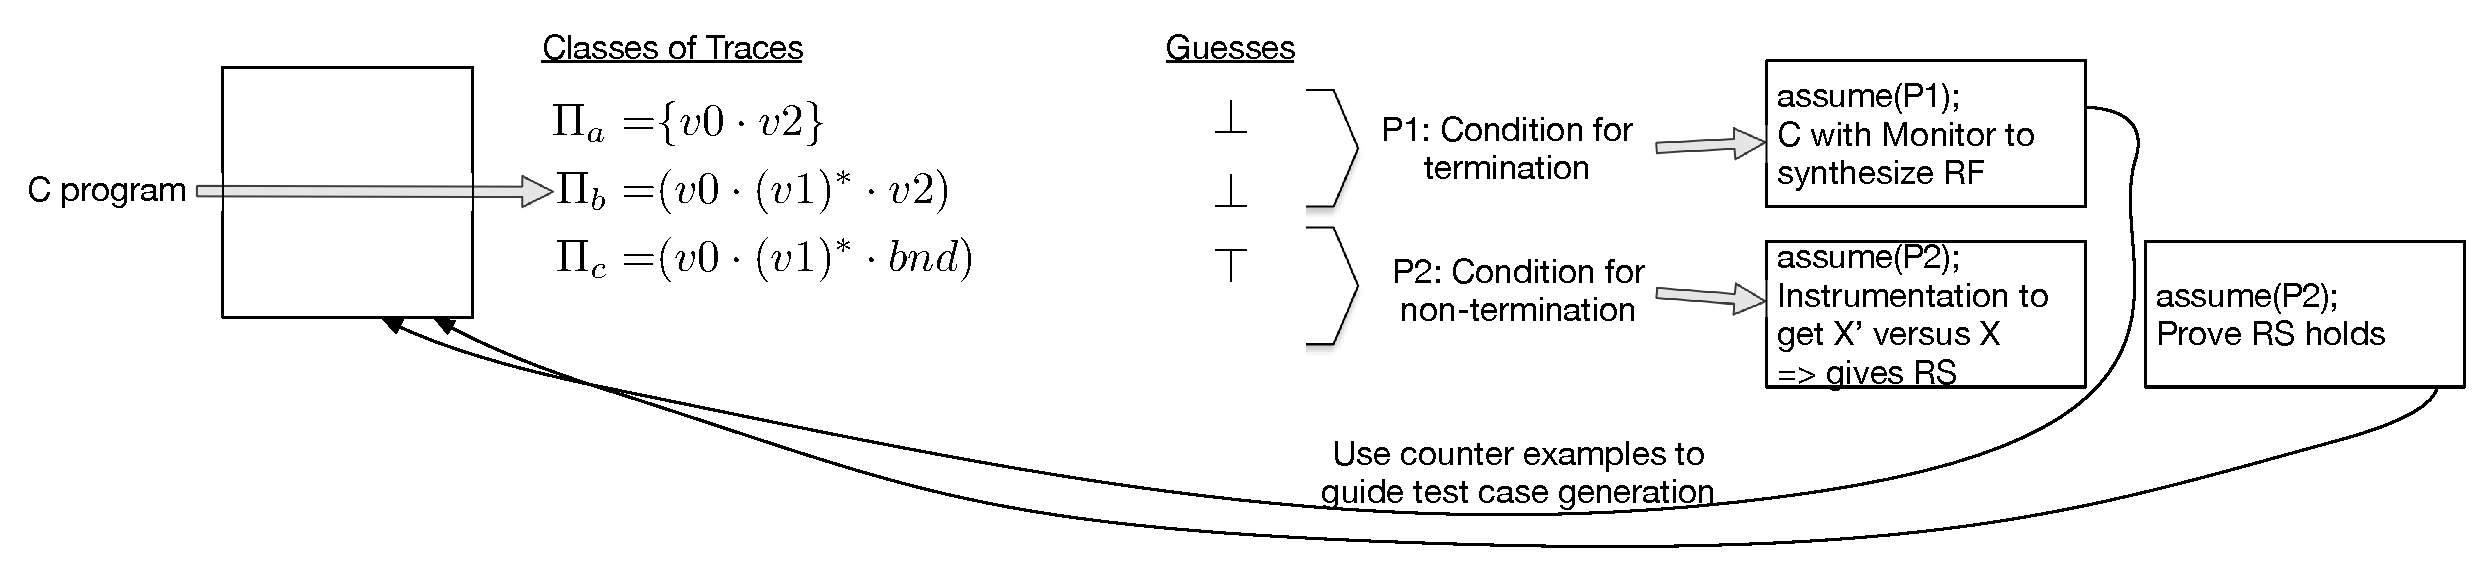
\includegraphics[width=4.5in]{boxes.eps}

\end{center}

\subsection{Expressiveness}

complciated functions like sin, exp, etc.

abstraction

\end{document}

